\id{IRSTI 82.33.13}{}

{\bfseries IMPROVING THE ECONOMIC MECHANISM OF INVESTMENT ACTIVITY}

{\bfseries IN THE REGION}

\footnote{}{\bfseries А. Tursyn\textsuperscript{\envelope }}
\begin{figure}[H]
	\centering
	
\includegraphics[width=0.8\textwidth]{media/ekon/image1}
	\caption*{}
\end{figure}

\textsuperscript{1}A.S.
\begin{figure}[H]
	\centering
	
\includegraphics[width=0.8\textwidth]{media/ekon/image1}
	\caption*{}
\end{figure}

\begin{figure}[H]
	\centering
	
\includegraphics[width=0.8\textwidth]{media/ekon/image1}
	\caption*{}
\end{figure}


{\bfseries \textsuperscript{1} A.A.Alzhanova}
\begin{figure}[H]
	\centering
	
\includegraphics[width=0.8\textwidth]{media/ekon/image1}
	\caption*{}
\end{figure}

\textsuperscript{3}
\begin{figure}[H]
	\centering
	
\includegraphics[width=0.8\textwidth]{media/ekon/image1}
	\caption*{}
\end{figure}


\emph{\textsuperscript{1}M. Auezov South Kazakhstan University,
Shymkent, Kazakhstan,}

\emph{\textsuperscript{2}Peoples'{} Friendship University
named after Academician A.Kuatbekov, Astana, Kazakhstan,}

\emph{\textsuperscript{3}Narxoz University}

\emph{{\bfseries \textsuperscript{\envelope }}Corresponding author:
\href{mailto:asilxan.janadilov@mail.ru}{\nolinkurl{asilxan.janadilov@mail.ru}}}

Enhancing the economic and organizational framework of the
region' s investment activity is essential to
guaranteeing long-term economic expansion and raising the
competitiveness of Kazakhstani regions. A key component of a
region' s successful growth in the face of global
competition and shifting global markets is its capacity to draw in and
use investments. With its abundant natural resources, Kazakhstan is
working to create a new economic model that emphasizes enhancing the
investment climate and expanding the contribution of private capital to
regional economies.

The theoretical underpinnings and real-world strategies for enhancing
the economic and organizational mechanisms of investment activity are
covered in the essay. In order to draw investment to the areas, the
current institutional and legislative frameworks as well as financial
incentives were examined and analyzed. An evaluation of the
state' s present business-state engagement mechanisms and
assistance programs is conducted. The main issues impeding the
successful execution of investment projects have been identified, and
these include inadequate funding, a lack of cooperation between
businesses and government organizations, and the digitization of
investment management.

Particular emphasis is placed on global experience, as demonstrated by
the cases of South Korea and Finland, where the implementation of
creative investment management techniques has sped up regional economic
expansion. Using the study as a basis, methodological suggestions are
made to enhance the economic and organizational mechanism of investment
activities. This would boost investment inflow and guarantee the
sustained development of Kazakhstan areas.

{\bfseries Keywords:} investment activity, organizational and economic
mechanism, government support, regional policy, financial incentives,
digitalization, investment climate, sustainable development.

{\bfseries АЙМАҚТАҒЫ ИНВЕСТИЦИЯЛЫҚ ҚЫЗМЕТТІҢ ЭКОНОМИКАЛЫҚ}

{\bfseries МЕХАНИЗМІН ЖЕТІЛДІРУ}

\textsuperscript{1}А.Р.Тұрсын\textsuperscript{\envelope },
\textsuperscript{1}А.С.Тулеметова, \textsuperscript{2}Г.С.Бердибекова,

\textsuperscript{1}А.А.Альжанова, \textsuperscript{3}Е.К.Тоимбетов

\emph{\textsuperscript{1}Южно-Казахстанский университет им. М. Ауэзова,
Шымкент, Казахстан,}

\emph{\textsuperscript{2}Университет дружбы народов им академика А.
Куатбекова, Шымкент, Казахстан,}

\emph{\textsuperscript{3}Университет Нархоз,}

\emph{е-mail
\href{mailto:asilxan.janadilov@mail.ru}{\nolinkurl{asilxan.janadilov@mail.ru}}}

Өңірдің инвестициялық қызметінің ұйымдастырушылық-экономикалық тетігін
жетілдіру тұрақты экономикалық өсуді қамтамасыз ету және Қазақстандағы
өңірлердің бәсекеге қабілеттілігін арттыру үшін негізгі фактор болып
табылады. Жаһандық бәсекелестік пен әлемдік нарықтардағы өзгерістер
жағдайында өңірлердің инвестицияларды тиімді тарту және пайдалану
қабілеті олардың табысты дамуының айқындаушы элементіне айналады.
Қазақстан бай табиғи әлеуетке ие бола отырып, инвестициялық ахуалды
жақсартуға және өңірлердің экономикасындағы жеке капиталдың рөлін
арттыруға негізделген экономиканың жаңа моделін дамытуға ұмтылады.

Мақалада инвестициялық қызметтің ұйымдастырушылық-экономикалық
механизмін жетілдірудің теориялық негіздері мен практикалық тәсілдері
қарастырылады. Өңірлерге инвестициялар тартуға ықпал ететін қолданыстағы
құқықтық және институционалдық жағдайларды, сондай-ақ қаржылық
ынталандыруларды зерделеу және талдау жүргізілді. Қолданыстағы
мемлекеттік қолдау бағдарламалары мен мемлекет пен бизнестің өзара
іс-қимыл тетіктеріне шолу жасалды. Қаржыландырудың жеткіліксіздігін,
мемлекеттік органдар мен бизнес арасындағы үйлестірудің әлсіздігін,
сондай-ақ инвестицияларды басқаруды цифрландыруды қоса алғанда,
инвестициялық жобаларды тиімді іске асыруға кедергі келтіретін түйінді
проблемалар анықталды.

Инвестицияларды басқарудың инновациялық тетіктерін енгізу өңірлердің
экономикалық өсуін жеделдетуге алып келген Финляндия мен Оңтүстік
Кореяның мысалдары сияқты халықаралық тәжірибеге ерекше назар аударылды.
Жүргізілген талдау негізінде инвестициялық қызметтің
ұйымдастырушылық-экономикалық тетігін жетілдіру бойынша әдіснамалық
ұсынымдар ұсынылды, бұл инвестициялар ағынын ұлғайтуға және Қазақстан
өңірлерінің тұрақты дамуын қамтамасыз етуге мүмкіндік береді.

{\bfseries Түйін сөздер:} инвестициялық қызмет, ұйымдастыру-экономикалық
тетік, мемлекеттік қолдау, өңірлік саясат, қаржылық ынталандыру,
цифрландыру, инвестициялық ахуал, орнықты даму.

{\bfseries СОВЕРШЕНСТВОВАНИЕ ЭКОНОМИЧЕСКОГО МЕХАНИЗМА ИНВЕСТИЦИОННОЙ
ДЕЯТЕЛЬНОСТИ В РЕГИОНЕ}

\footnote{}А.Р.Турсын\textsuperscript{\envelope },
\textsuperscript{1}А.С.Тулеметова, \textsuperscript{2}Г.С.Бердибекова,

\textsuperscript{1} А.А.Альжанова, \textsuperscript{3}Е.К.Тоимбетов

\emph{\textsuperscript{1}М.Әуезов атындағы Оңтүстік Қазақстан
университеті, Шымкент, Қазақстан,}

\emph{\textsuperscript{2}Академик Ә.Қуатбеков атындағы Халықтыр достығы
университеті,}

\emph{\textsuperscript{3}Нархоз университеті}

\emph{e-mail
\href{mailto:asilxan.janadilov@mail.ru}{\nolinkurl{asilxan.janadilov@mail.ru}}}

Совершенствование организационно-экономического механизма инвестиционной
деятельности региона является ключевым фактором для обеспечения
устойчивого экономического роста и повышения конкурентоспособности
регионов в Казахстане. В условиях глобальной конкуренции и изменений на
мировых рынках, способность регионов эффективно привлекать и
использовать инвестиции становится определяющим элементом их успешного
развития. Казахстан, обладая богатым природным потенциалом, стремится к
развитию новой модели экономики, основанной на улучшении инвестиционного
климата и повышении роли частного капитала в экономике регионов.

В статье рассматриваются теоретические основы и практические подходы к
совершенствованию организационно-экономического механизма инвестиционной
деятельности. Проведено изучение и анализ существующих правовых, и
институциональных условий, а также финансовых стимулов, способствующих
привлечению инвестиций в регионы. Проведен обзор действующих программ
государственной поддержки и механизмов взаимодействия государства и
бизнеса. Выявлены ключевые проблемы, препятствующие эффективной
реализации инвестиционных проектов, включая недостаточное
финансирование, слабую координацию между государственными органами и
бизнесом, а также цифровизацию управления инвестициями.

Особое внимание уделено международному опыту, такому как примеры
Финляндии и Южной Кореи, где внедрение инновационных механизмов
управления инвестициями привело к ускорению экономического роста
регионов. На основе проведенного анализа предложены методологические
рекомендации по совершенствованию организационно-экономического
механизма инвестиционной деятельности, что позволит увеличить приток
инвестиций и обеспечить устойчивое развитие регионов Казахстана.

{\bfseries Ключевые слова:} инвестиционная деятельность;
организационно-экономический механизм; государственная поддержка;
региональная политика; финансовые стимулы; цифровизация; инвестиционный
климат; устойчивое развитие.

{\bfseries Introduction.} Enhancing the organizational and economic
mechanisms of investment activity in the region is becoming a pressing
problem in light of the world economy' s volatility and
fast globalization. {[}1{]} Investments are essential for maintaining
steady economic growth, generating employment, and raising
people' s standard of living. An integrated strategy that
considers both the theoretical and practical facets of investment
activity is necessary for effective investment recruitment.

The success of present plans may be evaluated, flaws can be found, and
new ways to boost investment activity can be developed by analyzing the
regional level' s current investment management systems.
The effects of digitization on economic and organizational systems
should get particular attention as they provide new opportunities for
improving the efficiency and transparency of investment processes
{[}2{]}.

In order to determine the main elements influencing the growth in the
amount of investments and their efficient use, this research aims to
assess and analyze the current organizational and economic processes of
investment activity in the regions.

A survey of earlier research indicates that long-term economic growth
requires efficient investment processes. However, many locations still
confront significant challenges in spite of government assistance and
efforts to enhance the business climate. These include inadequate
financial resources, excessive investor risks, and a lack of cooperation
between the private sector and various governmental levels.

The study looks at the theoretical underpinnings of investment activity
and evaluates how investment management is being practiced in various
Kazakhstani areas. The operations of specialist organizations,
investment assistance initiatives, and communications with global
financial institutions are given particular consideration. An empirical
study will be carried out using the gathered statistical data on
unemployment, economic growth, and investment attractiveness. Based on
surveys and interviews with government and industry leaders, the issues
and obstacles faced by investors are also examined. Consequently,
suggestions for enhancing the economic and organizational mechanism of
investment activities will be developed, along with ideas for the growth
of international collaboration to boost the competitiveness of
Kazakhstan' s regions {[}3{]}.

{\bfseries Materials and methods.} In the current world, attaining
sustained economic growth in the regions depends heavily on efficient
investment management. The organizational and financial systems that
support investment process optimization are covered in this article.
With a focus on introducing innovations and utilizing global expertise,
the research examines the theoretical and practical elements of
improving these systems.

The study employs a comparative methodology in addition to statistical
and economic analysis. Data from official sources, including the Agency
for Statistics and the Ministry of National Economy, were examined in
order to evaluate the current level of investment activity in
Kazakhstan. Indicators pertaining to the amount of funding allocated to
research and development (R\&D) and the proportion of innovative
businesses across different areas were the primary emphasis. Statistics
posted on the Statistics Agency' s official website
corroborate the good trend in Kazakhstan' s GDP growth
rate {[}1{]}.

A data visualization was made to show the correlation between the amount
of money invested in creative ventures and the GDP growth rate in
different parts of Kazakhstan. On the figure 1 graph:

\begin{itemize}
\item
  The amount of investments in millions is shown in the blue bar graph.
\item
  The GDP growth rate is displayed as a percentage in the orange line
  graph.
\end{itemize}

The association between investment activity and economic development in
various places may be readily shown thanks to this representation (Fig.
1).

\begin{figure}[H]
	\centering
	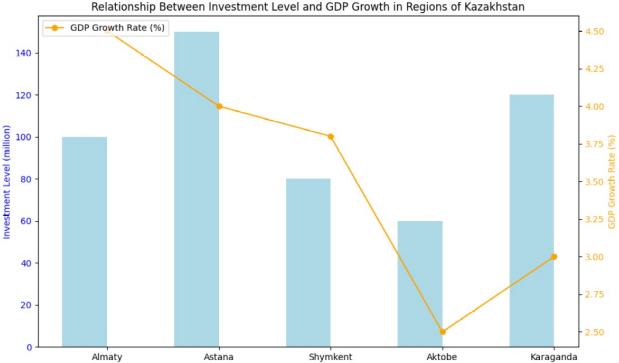
\includegraphics[width=0.8\textwidth]{media/ekon/image3}
	\caption*{}
\end{figure}


{\bfseries Fig. 1 - Correlation between Investment Level and GDP Growth
Rates in Regions of Kazakhstan}

The GDP growth rates and investment levels in
Kazakhstan' s five major regions are shown in Table 1.
These statistics enable a more thorough comprehension of the influence
of investments on regional economic development and validate the
association seen in the graph.

% \begin{longtable}[]{@{}
%   >{\raggedright\arraybackslash}p{(\columnwidth - 4\tabcolsep) * \real{0.3403}}
%   >{\raggedright\arraybackslash}p{(\columnwidth - 4\tabcolsep) * \real{0.3595}}
%   >{\raggedright\arraybackslash}p{(\columnwidth - 4\tabcolsep) * \real{0.3003}}@{}}
% \toprule\noalign{}
% \begin{minipage}[b]{\linewidth}\raggedright
% Region
% \end{minipage} & \begin{minipage}[b]{\linewidth}\raggedright
% Investment level (million)
% \end{minipage} & \begin{minipage}[b]{\linewidth}\raggedright
% GDP growth rate (\%)
% \end{minipage} \\
% \midrule\noalign{}
% \endhead
% \bottomrule\noalign{}
% \endlastfoot
% Almaty & 100 & 4.5 \\
% Astana & 150 & 4.0 \\
% Shymkent & 80 & 3.8 \\
% Aktobe & 60 & 2.5 \\
% Karaganda & 120 & 3.0 \\
% \end{longtable}

{\bfseries Table 1- GDP growth rates and investment levels by Kazakhstan's
regions}

The study' s examination of government assistance
initiatives for innovative endeavors was a significant component. The
Business Roadmap 2025 initiative, which offers funding for small and
medium-sized businesses, including creative firms, is specifically under
consideration. Information on the program' s outcomes was
gathered from publications on investment project outcomes and Ministry
of National Economy papers {[}2{]}. The high efficiency of public
financing of innovative ventures was supported by a study of worldwide
experience, including instances from Finland and South Korea. This was
also examined in previous scholarly studies {[}3{]}.

The study employed a range of sources to guarantee the validity and
applicability of the findings. These include information on the
intricacies of constructing these mechanisms and scholarly studies that
outline functional models of the organizational and economic mechanism
of investment management. Significant significance is placed on
statistical data released by the Statistics Agency that show the
dynamics of investments and how they affect economic indicators {[}4{]}.

The study' s examination of government assistance
initiatives for innovative endeavors was a significant component. The
Business Roadmap 2025 initiative, which offers funding for small and
medium-sized businesses, including creative firms, is specifically under
consideration. Information on the program' s outcomes was
gathered from publications on investment project outcomes and Ministry
of National Economy reports. The high effectiveness of public financing
of innovative ventures was validated by a review of worldwide
experience, including instances from Finland and South Korea. This was
also examined through existing scholarly studies {[}5{]}.

Throughout the study, a significant data visualization was produced that
showed the relationship between the amount of money invested in creative
enterprises and the GDP growth rate in different Kazakhstani areas.
Visual graphs enabled the analysis' s findings to be
visually represented and conclusions on the connection between economic
development and investment activity to be drawn {[}6{]}.

This study' s methodology highlights the necessity of
enhancing investment management' s organizational and
economic mechanisms through an integrated strategy that incorporates
both theoretical and practical elements. This will help the government
regulate and improve the investment climate in
Kazakhstan' s regions more effectively {[}7{]}.

{\bfseries Results and discussions.} The study' s findings
supported the crucial role that innovation plays in the economic growth
of Kazakhstan' s various regions, highlighting both
notable achievements and important obstacles that the nation must
overcome in order to create an inventive economy. According to the data,
areas with a high concentration of creative ventures have faster rates
of sustainability and economic growth.

A detailed overview of Almaty' s innovation activities
over the past three years shows significant and steady progress in both
economic growth and investment dynamics. In 2021, the gross regional
product (GRP) of Almaty grew by 3.8\%, which was a marked improvement
due to the constant influx of investments aimed at innovation. This
trend continued in 2022, when GDP growth rose to 4.2\%, further boosted
by increased financial allocations for innovation-oriented initiatives.
By 2023, the region' s GRP grew by 4.5\%, which indicates
the effectiveness of the strategic investment policy and the development
of the innovation ecosystem {[}8{]}.

The dynamics of investment in innovation once again confirms this thesis
about growth. In 2021, the volume of investments in innovation amounted
to \$85 million, increasing to 92 million in 2022. By 2023, these
investments will reach 100 million, which indicates steady annual growth
due to targeted government policies and a favorable business climate.
This progress highlights the key role of financial support mechanisms
and the growing confidence of private and public stakeholders in
Almaty' s innovative potential.

These changes indicate a change in the economic landscape of Almaty,
where innovation is a key factor in sustainable development. The
region' s ability to attract and effectively allocate
resources for innovative projects not only improves its economic
performance, but also serves as a reference point for other regions of
Kazakhstan. Using technological and infrastructural advantages, Almaty
demonstrates how strategic investments can contribute to the development
of a sustainable and competitive regional economy {[}9{]}.

Visualization of these tables clearly demonstrates the relationship
between investment activity and economic growth. The linear graph
illustrating the growth of GRP from 2021 to 2023 highlights the steady
upward trend in economic indicators (Fig 2).

\begin{figure}[H]
	\centering
	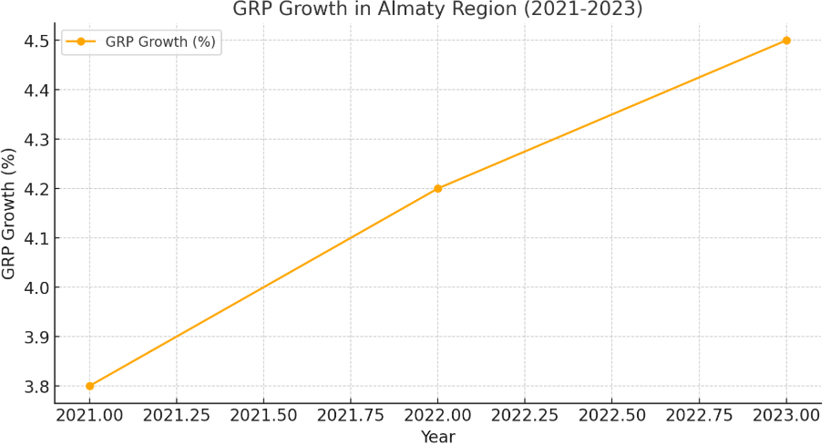
\includegraphics[width=0.8\textwidth]{media/ekon/image4}
	\caption*{}
\end{figure}


{\bfseries Fig.2 - GRP Growth in Almaty Region (2021-2023)}

Similarly, the histogram comparing investments in innovation over the
same period shows a gradual increase in financial investments, which
confirms the region' s commitment to stimulating
innovation (Fig. 3).

\begin{figure}[H]
	\centering
	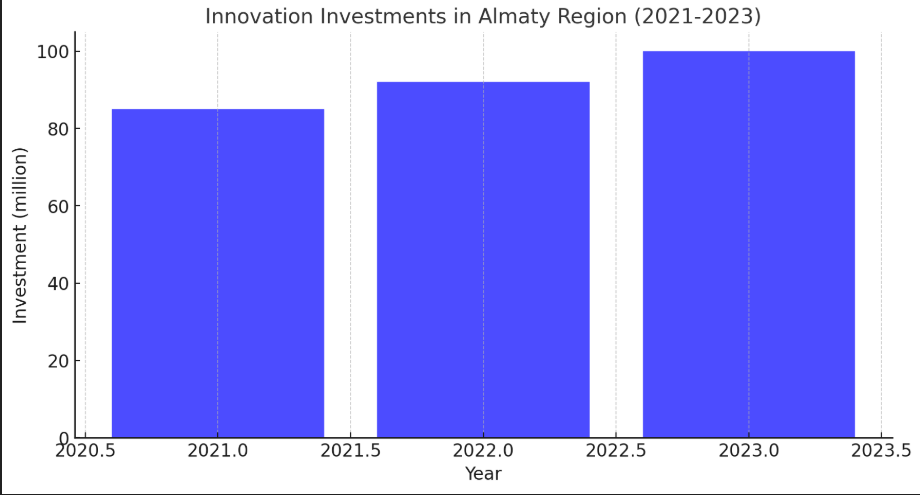
\includegraphics[width=0.8\textwidth]{media/ekon/image5}
	\caption*{}
\end{figure}


{\bfseries Fig.3 - Innovation Investments in Almaty Region (2021-2023)}

This analysis confirms the need for continuous investment in innovation
as the cornerstone of regional development. It highlights the importance
of aligning financial resources, policy frameworks, and infrastructure
support to maximize the economic potential of innovation. The experience
of Almaty provides a compelling example of the wider application of
these strategies throughout Kazakhstan, offering valuable insights into
the mechanisms that drive regional economic transformation.

For instance, Almaty, a pioneer in innovative activity, had a 4.5\%
growth in its gross regional product (GRP) in 2023, which is much
greater than Kazakhstan' s average growth rate of 3.3\%
{[}10{]}. These findings demonstrate how effective innovation
investments are as a means of promoting regional development. The
existence of scientific and technical parks in the area is significant
here as it fosters an environment that is conducive to startups and
innovative businesses.

International experience also supports this tendency. GDP growth often
surpasses 2\% per year in Finland, where government support for
innovation is a key component of economic strategy. This is linked to
active expenditures in R\&D and tight collaboration between industry and
science {[}11{]}. By using this experience, Kazakhstan may lessen
interregional gaps and promote a more equitable distribution of economic
advantages among regions. The relationship between academic institutions
and the private sector is given particular consideration in order to
successfully commercialize scientific advancements.

Nonetheless, the study identified important obstacles that restrict
Kazakhstan' s capacity for creative growth. The lack of
funding is still one of the primary issues; even though investments have
increased, they are still insufficient by global standards. Only 0.13\%
of GDP was allocated to research and development in 2023, which is much
less than what is done in OECD nations {[}12{]}. This restricts the
potential for the introduction of innovations in industry and the
development of new technologies.

Effective execution of new initiatives is hampered not just by a lack of
finance but also by a lack of collaboration between scientific
institutions and industry. Just 12\% of governmental scientific
initiatives in Kazakhstan are carried out in collaboration with industry
{[}13{]}. However, the proportion of marketable scientific advancements
in the US is far greater, highlighting the significance of collaboration
between industry and science for the effective application of
breakthroughs. The State has to pay more attention to this issue and
provide incentives for these kinds of exchanges. A SWOT analysis (Table.
2), which summarizes the main conclusions of this study, was carried out
in order to gain a better understanding of Kazakhstan' s
innovation environment and future prospects.

{\bfseries Table. 2 -- SWOT analysis result}

% \begin{longtable}[]{@{}
%   >{\raggedright\arraybackslash}p{(\columnwidth - 2\tabcolsep) * \real{0.5195}}
%   >{\raggedright\arraybackslash}p{(\columnwidth - 2\tabcolsep) * \real{0.4805}}@{}}
% \toprule\noalign{}
% \begin{minipage}[b]{\linewidth}\raggedright
% {\bfseries Strengths}
% \end{minipage} & \begin{minipage}[b]{\linewidth}\raggedright
% {\bfseries Weaknesses}
% \end{minipage} \\
% \midrule\noalign{}
% \endhead
% \bottomrule\noalign{}
% \endlastfoot
% Robust expansion in areas with a high concentration of creative
% businesses (e.g., Almaty' s GRP growth) & 0.13\% of GDP
% is spent on R\&D, which is far less than the OECD average \\
% The presence of technical and scientific parks that support startup
% settings & Only 12\% of government programs include industry and
% research organizations working together \\
% Shown relationship between GDP growth and government funding for
% innovation in global settings (e.g., Finland, South Korea) & Too little
% money and resources for new projects \\
% \end{longtable}

% \begin{longtable}[]{@{}
%   >{\raggedright\arraybackslash}p{(\columnwidth - 2\tabcolsep) * \real{0.5223}}
%   >{\raggedright\arraybackslash}p{(\columnwidth - 2\tabcolsep) * \real{0.4777}}@{}}
% \toprule\noalign{}
% \begin{minipage}[b]{\linewidth}\raggedright
% {\bfseries Opportunities}
% \end{minipage} & \begin{minipage}[b]{\linewidth}\raggedright
% {\bfseries Threats}
% \end{minipage} \\
% \midrule\noalign{}
% \endhead
% \bottomrule\noalign{}
% \endlastfoot
% Possibility of improving regional development by increasing R\&D
% spending (aiming for at least 1\% of GDP) & Low investment levels might
% impede technological advancement and innovation \\
% Growth of technology parks and incubators, particularly in developing
% regions & Increased interregional inequalities might result from
% inadequate assistance for less developed areas \\
% Financial assistance and tax breaks for the commercial sector Innovation
% might be sparked via R\&D & Competition from other countries that have
% more active financing and policies for innovation \\
% \end{longtable}

In light of the completed study, the following recommendations may be
made for the development of Kazakhstan' s creative
economy.

The effective growth of an innovative economy requires an integrated
approach that includes infrastructure development, government backing,
and private sector stimulation, according to an examination of global
experience. For instance, Kazakhstan can benefit from studying South
Korea' s experience, where substantial economic
development has resulted from aggressive government backing for
innovation. South Korea has become one of the world leaders in terms of
innovative activity because of the specific attention given to the
development of research parks and the training of competent individuals
{[}14{]}.

In order for innovations to be successfully implemented in Kazakhstan,
the present science and technology policy must be reviewed with an eye
toward successful foreign practices. This entails raising the proportion
of funds allocated to research and development, creating a nationwide
network of technology parks and incubators, and enhancing collaboration
between industry and academia.

The following suggestions for the advancement of
Kazakhstan' s creative economy may be made in light of
the study that has been done:

\begin{enumerate}
\def\labelenumi{\arabic{enumi}.}
\item
  A rise in R\&D spending to at least 1\% of GDP, which would greatly
  enhance the number of chances for new technology research and
  development.
\item
  One important step to guarantee an equitable distribution of
  innovation activity, particularly in less developed areas, will be to
  expand the number of technology parks and incubators around the
  nation.
\item
  The percentage of private investment in R\&D will rise with the
  implementation of tax breaks and other forms of financial assistance
  for businesses that make innovative investments.
\item
  Scientific advancements will be commercialized and introduced into
  industry more quickly if platforms and programs for interaction
  between universities and businesses are established.
\end{enumerate}

By putting these policies into place, Kazakhstan will be able to lessen
regional inequalities, boost its competitiveness in the international
market, and hasten the growth of an innovative economy.

Applying the finest worldwide techniques that have been modified for
local circumstances can guarantee the regions'{}
efficient growth, enhance the investment climate, and raise the
nation' s competitiveness abroad.

{\bfseries Conclusions.} This study' s goals were to examine
how innovation affects the economic development of
Kazakhstan' s various regions and to research strategies
for fostering innovation through infrastructure and government programs.
Throughout the project, techniques for evaluating the contribution of
investment activity to regional development, examining the experiences
of other nations, and analyzing economic indicators were applied.

The study verified that the economic growth of
Kazakhstan' s regions is significantly influenced by
innovative activity. Higher rates of sustainability and economic
development are found in areas that aggressively adopt cutting-edge
technology. There is a clear correlation between the degree of
innovation and economic advancement, as evidenced by the greater growth
rates of gross regional product (GRP) in areas with high rates of
investment activity in creative initiatives. This result reaffirms that
in order to guarantee sustained growth, new projects at the regional
level require a methodical approach.

The study' s findings also demonstrate that creative
approaches must be incorporated into comprehensive socioeconomic
development plans for areas to flourish successfully. Innovations should
be included into each region' s long-term development
plan rather than being a local endeavor. In addition to encouraging the
growth of innovative businesses, infrastructure development, the
establishment of technology parks and business incubators, and startup
assistance would help improve economic indices like employment and GRP
growth.

Specialized infrastructure, such as science and technology parks,
incubators, and accelerators, is required for the successful application
of creative ideas. These arrangements have the capacity to draw in
private capital for creative projects, which will advance the business
climate and quicken regional economic expansion. Experience from other
countries, such as the US and Israel, shows that assisting new
businesses with these kinds of arrangements speeds up the development
and commercialization of scientific discoveries. Similar initiatives
should be put in place in Kazakhstan to help creative projects at every
level of their growth.

According to an examination of global experience, nations like the US
and Israel have had considerable success promoting innovation by
building the necessary infrastructure and offering government
assistance. It is wise to implement strategies including establishing
specialized technology parks, accelerators, and enhancing collaboration
between academic institutions, corporations, and governmental
organizations in Kazakhstan. This will make it possible to employ
resources more effectively in order to promote scientific research and
technology commercialization.

Kazakhstan is particularly affected by the necessity to establish
regional competence centers that would focus on cutting-edge ideas and
technology. These facilities will aid in the concentration of resources
and knowledge, facilitating more efficient research and development of
new technologies. Experience from other countries, such as Switzerland,
demonstrates that the establishment of such centers helps to boost the
regions'{} standing internationally and promote the
growth of important economic sectors. These centers can be set up in
areas of Kazakhstan that have a lot of promise for the growth of
cutting-edge sectors including biotechnology, IT, and green
technologies.

International scientific conferences and the growth of scientific
tourism may both be useful instruments for raising a
region' s standing internationally. The organization of
significant scientific and technological events promotes information
sharing, the development of global relationships, and the promotion of
innovation. China serves as an example of how well-run international
scientific conferences draw top specialists from around the globe and
aid in the creation of cutting-edge technology.

Bureaucracy and administrative obstacles can seriously impede corporate
growth and innovation. Experience from other countries, including New
Zealand, demonstrates that streamlining business registration processes
and using electronic services help to foster a positive business
environment and draw capital to creative enterprises. In order to lower
administrative obstacles for creative businesses and hasten the adoption
of new technology, Kazakhstan should pursue changes in this area.

The following actions might be suggested for the advancement of
Kazakhstan' s innovative economy in light of the data
collected:

\begin{itemize}
\item
  There will be more chances for research and development of new
  technologies if R\&D spending is increased to at least 1\% of GDP.
\item
  The creation of a nationwide network of technology parks and
  incubators to guarantee that innovation activity is distributed
  fairly, particularly in underdeveloped areas.
\item
  Increasing the proportion of private investment in R\&D by offering
  tax breaks and other forms of financial assistance to businesses
  making innovative investments.
\item
  Establishment of forums and initiatives to facilitate communication
  between academic institutions and businesses, which will hasten the
  process of commercializing scientific discoveries and integrating them
  into the marketplace.
\end{itemize}

Therefore, a thorough application of global knowledge that is tailored
to Kazakhstan' s unique circumstances can greatly boost
regional innovation activity and support economic expansion. By taking
these steps, the nation' s competitiveness in the
international market will be bolstered, the investment climate will be
improved, and the existing resources will be used more efficiently.

References

\begin{enumerate}
\def\labelenumi{\arabic{enumi}.}
\item
  Agentstvo Respubliki Kazahstan po statistike, Investicionnaya
  statistika - dinamicheskie ryadi. URL:
  \url{https://stat.gov.kz/ru/industries/business-statistics/stat-invest/dynamic-tables/}
  {[}in Russian{]}
\item
  Petrova, I. A., \& Krasnova, N. A. (2015). Organizatsionno
  ekonomicheskiy mehanizm upravleniya investitsionnoy deyatelnostyu
  diversifitsirovannogo agropredpriyatiya regiona. URL:
  \url{https://cyberleninka.ru/article/n/organizatsionno-ekonomicheskiy-mehanizm-upravleniya-investitsionnoy-deyatelnostyu-diversifitsirovannogo-agropredpriyatiya-regiona}
  {[}in Russian{]}
\item
  Tokarev, A. A. (2016). Organizacionno\_ekonomicheskii mehanizm
  regionalnogo razvitiya. Institut menedjmenta\_ marketinga i finansov.
  DOI
  \href{https://doi.org/10.17308/meps.2016.11/1526}{10.17308/meps.2016.11/1526}
  {[}in Russian{]}
\item
  Yandarbaeva, L. A., \& Sherkhova, M. H.
  Osobennosti-postroeniya-organizatsionno-ekonomicheskogo-mehanizma-upravleniya-investitsionnoy-deyatelnostyu//
  Estestvenno-gumanitarnye issledovanija-2020.-№28(2)- С.290-294. DOI
  10.24411/2309-4788-2020 {[}in Russian{]}
\item
  Nasrutdinov, M., Gadzhiev, M., \& Zaborovskaya, O. (2021). FOREIGN
  EXPERIENCE OF THE USE OF THE TOOLS OF THE REGIONAL POLICY OF
  MANAGEMENT OF INVESTMENT ACTIVITY OF THE TERRITORIES. Zarubezhnyj opyt
  ispol' zovaniya instrumentov
  regional' noj politiki upravleniya investicionnoj
  aktivnost' yu territorij. Fundamentalnie issledovaniya
  (3), 120--127. DOI
  \href{https://doi.org/10.17513/fr.42991}{/10.17513/fr.42991} {[}in
  Russian{]}
\item
  Kosovskikh E.A., \& Trifonov Yu.V. Funktsionalnaya model
  organizatsionno ekonomicheskogo mehanizma upravleniya regionalnoy
  investitsionnoy deyatelnostyu// Jekonomika i finansy. Vestnik
  Nizhegorodskogo universiteta
  im.N.I.Lobachevskogoju-2022.-№3.-S.183-185 URL:
  \url{https://cyberleninka.ru/article/n/funktsionalnaya-model-organizatsionno-ekonomicheskogo-mehanizma-upravleniya-regionalnoy-investitsionnoy-deyatelnostyu}
  {[}in Russian{]}
\end{enumerate}

7. Lapaeva M.G., Bajtljuv S.A.Organizacionno-jekonomicheskij mehanizm
upravlenija investicionnym processov v regione./Vestnik
OGU.-2006ju-T.1(2).-S.91-98.{[}in Russian{]}

\url{https://cyberleninka.ru/article/n/organizatsionno-ekonomicheskiy-mehanizm-upravleniya-investitsionnym-protsessom-v-regione}

8. Ekonomika torgovli. Dannie za 1990\_2023 godi \textbar{} Prognoz na
2024\_2026 godi Dannie za 1990\_2023 godi \textbar{} Prognoz na
2024\_2026 godi. URL:
\url{https://ru.tradingeconomics.com/kazakhstan/gdp}. (date of request
12.12.2024) {[}in Russian{]}

9.Investicionnaya statistika. URL:
\url{https://stat.gov.kz/ru/industries/business-statistics/stat-invest/publications/5203/}
(date of request 12.12.2024) {[}in Russian{]}

10. Korotkov G.E. Razrabotka organizacionno-jekonomicheskogo mehanizma
povyshenija investicionnoj
privlekatel'' nosti regiona.// Rossijskij
zhurnal menedzhmenta.-2023.-T.11(1).-S.251-260.{[}in Russian{]}

\href{https://doi.org/10.29039/2409-6024-2023-11-1-251-260}{DOI
10.29039/2409-6024-2023-11-1-251-260}

11. Dinamicheskie tablici po investiciyam. URL:
\url{https://stat.gov.kz/ru/industries/business-statistics/stat-invest/dynamic-tables/}
(date of request 12.12.2024) {[}in Russian{]}

12.Ministerstvo po investiciyam i razvitiyu Respubliki
Kazahstan.~(2023).~KGIR-2023:~Investitsii v ustoychivyy regionalnyy
rost.~URL:
\url{https://invest.gov.kz/ru/media-center/press-releases/kgir-2023-investitsii-v-ustoychivyy-regionalnyy-rost/}
(date of request 12.12.2024) {[}in Russian{]}

13.Ministerstvo po investiciyam i razvitiyu Respubliki Kazahstan.
(2023). KGIR-2023: Investitsii v ustoychivyy regionalnyy rost. URL:
\url{https://invest.gov.kz/ru/media-center/press-releases/kgir-2023-investitsii-v-ustoychivyy-regionalnyy-rost/2023}
. (date of request 12.12.2024) {[}in Russian{]}

14.Ministerstvo nacionalnoi publikacii po statistike investicii. (2024).
URL:
\url{https://stat.gov.kz/ru/industries/business-statistics/stat-invest/publications/182352/}
(date of request 12.12.2024) {[}in Russian{]}

\emph{{\bfseries Information about the authors}}

Tursyn A. R.-PhD student, South Kazakhstan University named after M.
Auezov, Shymkent{\bfseries ,} Kazakhstan,
e-mail{\bfseries :}\href{mailto:asilxan.janadilov@mail.ru}{\nolinkurl{asilxan.janadilov@mail.ru}};

Tulemetova A. S.-Candidate of Economic Sciences, South Kazakhstan
University named after M. Auezov, Shymkent, Kazakhstan,
e-mail:\href{mailto:aygul.tul.76@mail.ru}{\nolinkurl{aygul.tul.76@mail.ru}};

Alzhanova A. A. {\bfseries -} Candidate of economic sciences, docent of the
department "Economics" M. Auezov South Kazakhstan State University,
Shymkent, Kazakhstan, e-mail:
\href{mailto:aigolek@mail.ru}{\nolinkurl{aigolek@mail.ru}};

Berdibekova G. S. -- Candidate of Economic Sciences, senior-lecturer,
Peoples'{} Friendship University named after Academician
A.Kuatbekov, Shymkent, Kazakhstan, e-mail:
\href{mailto:Gulua240165@gmail.com}{\nolinkurl{Gulua240165@gmail.com}};

Toimbetov Ye. {\bfseries -}Graduate student, Narxoz University, Almaty,
Kazakhstan, e-mail:
\href{mailto:yerbolvt@gmail.com}{\nolinkurl{yerbolvt@gmail.com}}

\emph{{\bfseries Информация об авторах}}

Тұрсын А. Р.- PhD Докторант, Южно-Казахстанский университет им. М.
Ауэзова, г.Шымкент.Казахстан,
е-mail{\bfseries :}\href{mailto:asilxan.janadilov@mail.ru}{\nolinkurl{asilxan.janadilov@mail.ru}};

Тулеметова А.С.-Кандидат экономических наук, Южно-Казахстанский
университет им. М. Ауэзова, г.Шымкент.
Казахстан,е-mail:\href{mailto:aygul.tul.76@mail.ru}{\nolinkurl{aygul.tul.76@mail.ru}};

Альжанова A.A. {\bfseries -} кандидат экономических наук, доцент кафедры
«Экономика» Южно-Казахстанский университет им. М.Ауэзова, г. Шымкент,
Казахстан, е-mail:
\href{mailto:aigolek@mail.ru}{\nolinkurl{aigolek@mail.ru}};

Бердибекова Г.С. кандидат экономических наук, старший преподаватель,
Университет дружбы народов им.академика А. Куатбекова, Шымкент,
Казахстан, e-mail:
\href{mailto:Gulua240165@gmail.com}{\nolinkurl{Gulua240165@gmail.com}};

Тоимбетов Е.К.-Магистрант, Университет Нархоз, г.Алматы,
Казахстан,е-mail:
\href{mailto:yerbolvt@gmail.com}{\nolinkurl{yerbolvt@gmail.com}}